\documentclass[preprint,12pt,aps,pra,showkeys,amsmath,amssymb,superscriptaddress,floatfix]{revtex4-2}
\usepackage[T1]{fontenc}
\usepackage[utf8]{inputenc}
\usepackage{amsmath,amssymb,amsthm,mathtools,mathrsfs}
\usepackage{microtype,booktabs,enumitem}
\usepackage{xcolor,tikz,etoolbox}
\usepackage[skins,breakable]{tcolorbox}
\usepackage{needspace}
% Keep diagram geometry independent of REVTeX preprint body spacing.
\AtBeginEnvironment{tikzpicture}{\linespread{1}\selectfont}
\usetikzlibrary{arrows.meta,positioning,calc,fit,decorations.pathreplacing}
\usepackage{graphicx}
\usepackage{hyperref}

\definecolor{MMBlue}{RGB}{0,82,155}
\definecolor{MMOrange}{RGB}{200,80,0}
\tikzset{
 mmnode/.style={draw=MMBlue,rounded corners=2pt,fill=MMBlue!4,align=left,execute at begin node={\raggedright},text width=5cm,font=\fontsize{10}{12}\selectfont,inner sep=6pt},
 mmimport/.style={mmnode,draw=black!65,fill=black!4},
 mmcandidate/.style={mmnode,draw=MMOrange,dashed,fill=MMOrange!5},
 mmrejected/.style={mmnode,draw=black,densely dotted,fill=black!8},
 mmproof/.style={->,thick,MMBlue},
 mmflow/.style={->,semithick,black!70},
 mmrepair/.style={->,dashed,thick,MMOrange},
 mmcandidatearrow/.style={->,dashed,semithick,MMOrange},
 mmnote/.style={font=\scriptsize,fill=white,inner sep=2pt,align=center}}

\usepackage[section]{placeins}
\setlength{\emergencystretch}{3em}
\setlist{itemsep=3pt,topsep=4pt}
\newtheorem{theorem}{Theorem}[section]
\newtheorem{proposition}[theorem]{Proposition}
\newtheorem{lemma}[theorem]{Lemma}
\newtheorem{corollary}[theorem]{Corollary}
\theoremstyle{definition}
\newtheorem{definition}[theorem]{Definition}
\newtheorem{example}[theorem]{Example}
\theoremstyle{remark}
\newtheorem{remark}[theorem]{Remark}
% Avoid isolated statement headings and single-line paragraph fragments.
\BeforeBeginEnvironment{theorem}{\Needspace{6\baselineskip}}
\BeforeBeginEnvironment{definition}{\Needspace{5\baselineskip}}
\BeforeBeginEnvironment{proposition}{\Needspace{5\baselineskip}}
\BeforeBeginEnvironment{lemma}{\Needspace{5\baselineskip}}
\BeforeBeginEnvironment{corollary}{\Needspace{5\baselineskip}}
\clubpenalty=5000
\widowpenalty=5000
\newcommand{\R}{\mathbb R}\newcommand{\Z}{\mathbb Z}\newcommand{\N}{\mathbb N}
\newcommand{\Pa}{\operatorname{Pa}}\newcommand{\Desc}{\operatorname{Desc}}
\newcommand{\cl}{\operatorname{cl}}\newcommand{\cost}{\operatorname{cost}}
\newcommand{\status}{\operatorname{status}}
% Faculty cards: a visual rail groups the five faculties within one agent.
% The rail has no arrowhead and does not represent a proof dependency.
\newcommand{\mmfacultybadge}[1]{%
 \node[circle,draw=MMBlue,line width=1pt,fill=white,
 minimum size=7mm,inner sep=0pt,font=\sffamily\small\bfseries,text=MMBlue]
 at ([xshift=15pt,yshift=-15pt]frame.north west) {#1};}
\newcommand{\mmfacultyrail}{%
 \draw[MMBlue!80,line width=1pt]
 ([xshift=15pt,yshift=2pt]frame.north west)--
 ([xshift=15pt,yshift=-2pt]frame.south west);}
\newtcolorbox{mmfacultybox}[2]{enhanced,breakable,
 colback=MMBlue!4,colframe=MMBlue!4,boxrule=0pt,arc=3pt,
 left=39pt,right=9pt,top=4pt,bottom=4pt,
 before skip=2pt,after skip=2pt,
 fontupper=\small\linespread{1.1}\selectfont,
 overlay unbroken={\mmfacultyrail\mmfacultybadge{#1}},
 overlay first={\mmfacultyrail\mmfacultybadge{#1}},
 overlay middle={\mmfacultyrail},overlay last={\mmfacultyrail}}
\newcommand{\mmfaculty}[3]{%
 \begin{mmfacultybox}{#1}{#2}
 {\sffamily\bfseries\color{MMBlue}#2}\par\smallskip #3
 \end{mmfacultybox}}
\newcommand{\agent}[9]{%
 \Needspace{8\baselineskip}
 \subsubsection{#1}
 \noindent\textbf{Object.} #2\par
 \noindent\textbf{Role.} #3\par\smallskip
 \mmfaculty{E}{Ego}{#4}
 \mmfaculty{M}{Memory}{#5}
 \mmfaculty{I}{Intellect}{#6}
 \mmfaculty{S}{Sense}{#7}
 \mmfaculty{A}{Action}{#8}
 \smallskip\noindent #9\par}

\usepackage{longtable,array,calc}
\providecommand{\tightlist}{\setlength{\itemsep}{2pt}\setlength{\parskip}{0pt}}
\makeatletter
\def\frontmatter@abstract@produce{\par\addvspace{\frontmatter@preabstractspace}%
\begingroup\prep@absbox\unvbox\absbox\post@absbox\endgroup
\addvspace{\frontmatter@postabstractspace}}
\makeatother
\newcommand{\field}[2]{\par\smallskip\noindent\textbf{#1.} #2\par}
\setlength{\emergencystretch}{5em}
\AtBeginEnvironment{verbatim}{\small\linespread{1.0}\selectfont}


\hypersetup{colorlinks=true,linkcolor=MMBlue,urlcolor=MMBlue,pdfauthor={Dibakar Sigdel}}

\begin{document}

\title{Fejér's Theorem\\[4pt]\large An End-to-End Meta-Math Walkthrough}

\author{Dibakar Sigdel}

\affiliation{Mindverse Computing LLC, Lynnwood, WA 98087, USA}

\date{October 2026}

\begin{abstract}

A complete authored walkthrough of fejér's theorem, with explicit
mathematical contracts, local verification gates, and reusable exports.
The report presents the target theorem, declared imports, a dependency
graph, five-faculty node contracts, a continuous proof, a worked
example, and a hypothesis-repair audit. It is an authored mathematical
exposition, not a deployed-agent transcript or a formal proof-assistant
certificate.

\end{abstract}\maketitle\linespread{1.12}\selectfont

\noindent\textbf{HA-02 / Harmonic Analysis / Report v1}

\section{Target and import contract}

\begin{theorem}

If f is continuous and \(2\pi\)-periodic, the Cesàro means of its
Fourier partial sums converge uniformly to f:

\[\sigma_N f=\frac{S_0f+\cdots+S_Nf}{N+1},\qquad\|\sigma_Nf-f\|_\infty\to0.\]

Use normalized measure \(dt/(2\pi)\) on \([-\pi ,\pi ]\), coefficients
\(c_k=\int f(t)e^{-ikt}\,dt/(2\pi)\), and
\(S_nf(x)=\sum_{|k|\le n}c_ke^{ikx}\). The output concerns averaged
partial sums, not a promise about the raw \(S_n\).

\end{theorem}

\subsection{Foundations and permitted imports}

elementary exponential orthogonality, finite geometric sums, boundedness
and uniform continuity of continuous functions on a compact circle. All
kernel identities and convergence estimates are proved below.

\clearpage\section{Node interaction workflow}

\begin{center}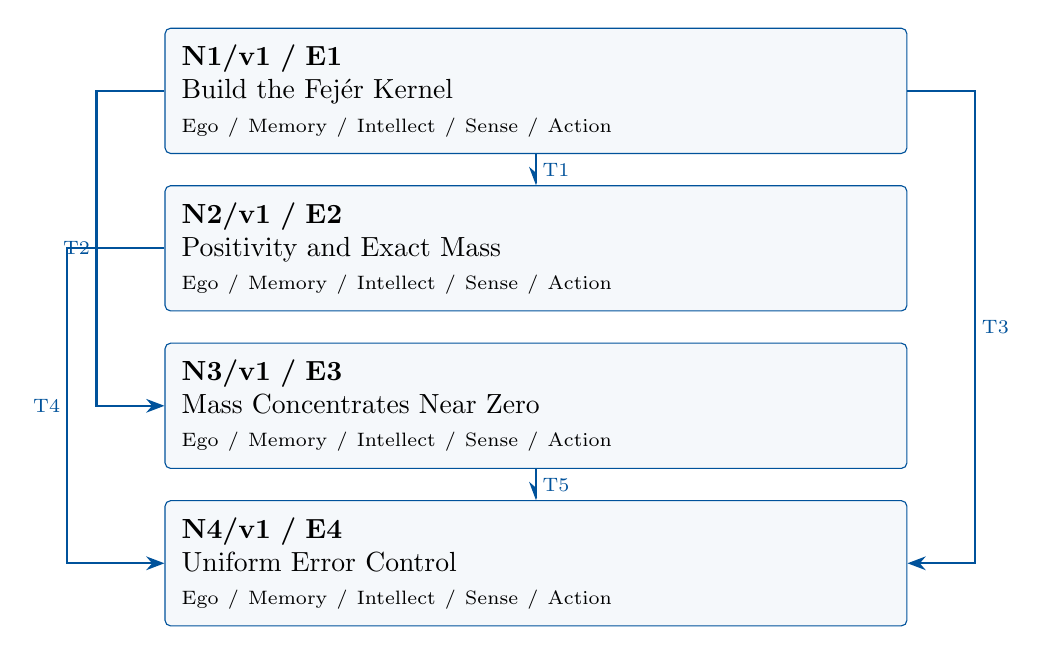
\begin{tikzpicture}[>=Stealth,x=1cm,y=1cm]

\node[mmnode,text width=9cm,minimum height=1.25cm] (N1) at (0,0.0) {\textbf{N1/v1 / E1}\\Build the Fejér Kernel\\{\scriptsize Ego / Memory / Intellect / Sense / Action}};

\node[mmnode,text width=9cm,minimum height=1.25cm] (N2) at (0,-2.0) {\textbf{N2/v1 / E2}\\Positivity and Exact Mass\\{\scriptsize Ego / Memory / Intellect / Sense / Action}};

\node[mmnode,text width=9cm,minimum height=1.25cm] (N3) at (0,-4.0) {\textbf{N3/v1 / E3}\\Mass Concentrates Near Zero\\{\scriptsize Ego / Memory / Intellect / Sense / Action}};

\node[mmnode,text width=9cm,minimum height=1.25cm] (N4) at (0,-6.0) {\textbf{N4/v1 / E4}\\Uniform Error Control\\{\scriptsize Ego / Memory / Intellect / Sense / Action}};

\draw[mmproof] (N1.south) -- node[mmnote,right] {T1} (N2.north);

\draw[mmproof] (N1.west) -- (-5.58,0) -- node[mmnote,left] {T2} (-5.58,-4) -- (N3.west);

\draw[mmproof] (N1.east) -- (5.58,0) -- node[mmnote,right] {T3} (5.58,-6) -- (N4.east);

\draw[mmproof] (N2.west) -- (-5.96,-2) -- node[mmnote,left] {T4} (-5.96,-6) -- (N4.west);

\draw[mmproof] (N3.south) -- node[mmnote,right] {T5} (N4.north);

\end{tikzpicture}\end{center}

Each box is one mathematical agent containing all five faculties. Blue
arrows carry the versioned exports listed below. The layout gives a
reading order; only drawn arrows assert dependencies. Diagnostic repair
is separate from the proof DAG.

\clearpage\subsection{Versioned evidence-transfer ledger}

\begingroup\small\linespread{1.05}\selectfont

\Needspace{5\baselineskip}\field{T1: N1/E1/v1 to N2}{\(\sigma_N f=f*K_N\) and \(K_N(t)=\frac1{N+1}|\sum_{j=0}^N e^{ijt}|^2\).}

\field{Receiving activity}{N2: Positivity and Exact Mass}

\field{Compatibility}{Use the same mathematical objects and hypotheses as the source export.
Receiving contract: N1/E1 and finite exponential orthogonality.}

\Needspace{5\baselineskip}\field{T2: N1/E1/v1 to N3}{\(\sigma_N f=f*K_N\) and \(K_N(t)=\frac1{N+1}|\sum_{j=0}^N e^{ijt}|^2\).}

\field{Receiving activity}{N3: Mass Concentrates Near Zero}

\field{Compatibility}{Use the same mathematical objects and hypotheses as the source export.
Receiving contract: N1/E1, with a fixed distance \(\delta\) from zero on
the circle.}

\Needspace{5\baselineskip}\field{T3: N1/E1/v1 to N4}{\(\sigma_N f=f*K_N\) and \(K_N(t)=\frac1{N+1}|\sum_{j=0}^N e^{ijt}|^2\).}

\field{Receiving activity}{N4: Uniform Error Control}

\field{Compatibility}{Use the same mathematical objects and hypotheses as the source export.
Receiving contract: N1/E1, N2/E2, N3/E3, and uniform continuity on the
compact circle.}

\Needspace{5\baselineskip}\field{T4: N2/E2/v1 to N4}{\(K_N\ge0\) and \(\int_{-\pi}^{\pi}K_N(t)\,dt/(2\pi)=1\).}

\field{Receiving activity}{N4: Uniform Error Control}

\field{Compatibility}{Use the same mathematical objects and hypotheses as the source export.
Receiving contract: N1/E1, N2/E2, N3/E3, and uniform continuity on the
compact circle.}

\Needspace{5\baselineskip}\field{T5: N3/E3/v1 to N4}{\(\int_{\delta\le|t|\le\pi}K_N(t)\,dt/(2\pi)\le[(N+1)\sin^2(\delta/2)]^{-1}\)
for \(0<\delta<\pi\).}

\field{Receiving activity}{N4: Uniform Error Control}

\field{Compatibility}{Use the same mathematical objects and hypotheses as the source export.
Receiving contract: N1/E1, N2/E2, N3/E3, and uniform continuity on the
compact circle.}

\endgroup

\clearpage\section{Agent roles and five-faculty activities}\begingroup\small\linespread{1.05}\selectfont\setlist{itemsep=1pt,topsep=2pt}

\subsection{N1/v1: Build the Fejér Kernel}

\field{Object and role}{Build the Fejér Kernel. Establish the following local result:
\(\sigma_N f=f*K_N\) and \(K_N(t)=\frac1{N+1}|\sum_{j=0}^N e^{ijt}|^2\).}

\field{Inputs}{Normalized circle measure, Fourier coefficients, and finite geometric
sums.}

\mmfaculty{E}{Ego}{Own E1/v1: \(\sigma_N f=f*K_N\) and
\(K_N(t)=\frac1{N+1}|\sum_{j=0}^N e^{ijt}|^2\).}

\mmfaculty{M}{Memory}{Fourier conventions}

\mmfaculty{I}{Intellect}{Rewrite average as convolution}

\mmfaculty{S}{Sense}{Track N+1 and normalized measure}

\mmfaculty{A}{Action}{Carry out the numbered deductions and publish E1/v1 together with its
hypotheses and proof location.}

\smallskip\noindent\textbf{Numbered mathematical activities}

\begin{enumerate}[label=N1.\arabic*,leftmargin=3.4em]

\item Write each partial sum as convolution with its Dirichlet kernel.

\item Average the finite sums to obtain triangular Fourier weights.

\item Expand the squared finite exponential sum and derive the sine quotient,
with its continuous value at zero.

\end{enumerate}

\field{Export E1/v1}{\(\sigma_N f=f*K_N\) and \(K_N(t)=\frac1{N+1}|\sum_{j=0}^N e^{ijt}|^2\).}

\field{Acceptance gate}{Track N+1 and normalized measure Publish only after checking every
displayed deduction.}

\field{Targeted repair}{If the check fails, revise N1: Track N+1 and normalized measure Recheck
dependent nodes N2, N3, N4.}

\clearpage

\subsection{N2/v1: Positivity and Exact Mass}

\field{Object and role}{Positivity and Exact Mass. Establish the following local result:
\(K_N\ge0\) and \(\int_{-\pi}^{\pi}K_N(t)\,dt/(2\pi)=1\).}

\field{Inputs}{N1/E1 and finite exponential orthogonality.}

\mmfaculty{E}{Ego}{Own E2/v1: \(K_N\ge0\) and \(\int_{-\pi}^{\pi}K_N(t)\,dt/(2\pi)=1\).}

\mmfaculty{M}{Memory}{Orthogonality}

\mmfaculty{I}{Intellect}{Use squared finite sum}

\mmfaculty{S}{Sense}{Include value at zero}

\mmfaculty{A}{Action}{Carry out the numbered deductions and publish E2/v1 together with its
hypotheses and proof location.}

\smallskip\noindent\textbf{Numbered mathematical activities}

\begin{enumerate}[label=N2.\arabic*,leftmargin=3.4em]

\item Use the squared-sum identity for nonnegativity.

\item Integrate the finite Fourier expansion: only its constant coefficient
remains.

\item Deduce preservation of constants and the sup-norm contraction bound.

\end{enumerate}

\field{Export E2/v1}{\(K_N\ge0\) and \(\int_{-\pi}^{\pi}K_N(t)\,dt/(2\pi)=1\).}

\field{Acceptance gate}{Include value at zero Publish only after checking every displayed
deduction.}

\field{Targeted repair}{If the check fails, revise N2: Include value at zero Recheck dependent
nodes N4.}

\clearpage

\subsection{N3/v1: Mass Concentrates Near Zero}

\field{Object and role}{Mass Concentrates Near Zero. Establish the following local result:
\(\int_{\delta\le|t|\le\pi}K_N(t)\,dt/(2\pi)\le[(N+1)\sin^2(\delta/2)]^{-1}\)
for \(0<\delta<\pi\).}

\field{Inputs}{N1/E1, with a fixed distance \(\delta\) from zero on the circle.}

\mmfaculty{E}{Ego}{Own E3/v1:
\(\int_{\delta\le|t|\le\pi}K_N(t)\,dt/(2\pi)\le[(N+1)\sin^2(\delta/2)]^{-1}\)
for \(0<\delta<\pi\).}

\mmfaculty{M}{Memory}{Sine denominator bounds}

\mmfaculty{I}{Intellect}{Bound exterior mass}

\mmfaculty{S}{Sense}{Stay away from zero modulo \(2\pi\)}

\mmfaculty{A}{Action}{Carry out the numbered deductions and publish E3/v1 together with its
hypotheses and proof location.}

\smallskip\noindent\textbf{Numbered mathematical activities}

\begin{enumerate}[label=N3.\arabic*,leftmargin=3.4em]

\item Bound the sine numerator by one.

\item Bound the denominator below by \(\sin^2(\delta/2)\).

\item Integrate over a set of normalized measure at most one.

\end{enumerate}

\field{Export E3/v1}{\(\int_{\delta\le|t|\le\pi}K_N(t)\,dt/(2\pi)\le[(N+1)\sin^2(\delta/2)]^{-1}\)
for \(0<\delta<\pi\).}

\field{Acceptance gate}{Stay away from zero modulo \(2\pi\) Publish only after checking every
displayed deduction.}

\field{Targeted repair}{If the check fails, revise N3: Stay away from zero modulo \(2\pi\)
Recheck dependent nodes N4.}

\clearpage

\subsection{N4/v1: Uniform Error Control}

\field{Object and role}{Uniform Error Control. Establish the following local result:
\(\|\sigma_N f-f\|_\infty\to0\) for every continuous periodic \(f\).}

\field{Inputs}{N1/E1, N2/E2, N3/E3, and uniform continuity on the compact circle.}

\mmfaculty{E}{Ego}{Own E4/v1: \(\|\sigma_N f-f\|_\infty\to0\) for every continuous periodic
\(f\).}

\mmfaculty{M}{Memory}{Uniform continuity and boundedness}

\mmfaculty{I}{Intellect}{Split near and far errors}

\mmfaculty{S}{Sense}{Use one delta for all x}

\mmfaculty{A}{Action}{Carry out the numbered deductions and publish E4/v1 together with its
hypotheses and proof location.}

\smallskip\noindent\textbf{Numbered mathematical activities}

\begin{enumerate}[label=N4.\arabic*,leftmargin=3.4em]

\item Write the error as the convolution of the increment \(f(x-t)-f(x)\).

\item Choose one \(\delta\) controlling the near part uniformly in \(x\).

\item Bound the far part by \(2\|f\|_\infty\) times the tail mass and then
choose \(N\).

\end{enumerate}

\field{Export E4/v1}{\(\|\sigma_N f-f\|_\infty\to0\) for every continuous periodic \(f\).}

\field{Acceptance gate}{Use one delta for all x Publish only after checking every displayed
deduction.}

\field{Targeted repair}{If the check fails, revise N4: Use one delta for all x Withhold this
terminal result until its gate passes.}

\endgroup\clearpage\section{Continuous mathematical proof}\label{sec:proof}

\subsection{N1 --- Build the Fejér
Kernel}\label{n1-build-the-fejuxe9r-kernel}

The Dirichlet kernel is \(D_n(t)=\sum_{|k|\le n}e^{ikt}\). Finite
rearrangement gives

\[S_nf(x)=\int_{-\pi}^{\pi}f(x-t)D_n(t)\,\frac{dt}{2\pi}.\]

Averaging yields the same expression with

\[K_N(t)=\frac1{N+1}\sum_{n=0}^ND_n(t)=\sum_{|k|\le N}\left(1-\frac{|k|}{N+1}\right)e^{ikt}.\]

To obtain positivity, expand the square:

\[\left|\sum_{j=0}^Ne^{ijt}\right|^2=\sum_{j,l=0}^Ne^{i(j-l)t}=\sum_{|k|\le N}(N+1-|k|)e^{ikt}.\]

Thus

\[K_N(t)=\frac1{N+1}\left|\sum_{j=0}^Ne^{ijt}\right|^2=\frac1{N+1}\frac{\sin^2((N+1)t/2)}{\sin^2(t/2)}\]

for t not a multiple of \(2\pi\). The continuous value at zero is N+1.
This proves \(\sigma_Nf=f*K_N\) without any interchange of infinite
sums.

\subsection{N2 --- Positivity and Exact
Mass}\label{n2-positivity-and-exact-mass}

The squared-sum expression proves \(K_N\ge0\). Integrate its finite
Fourier expansion. Every nonzero exponential has normalized integral
zero, while the constant coefficient is 1. Hence

\[\int_{-\pi}^{\pi}K_N(t)\,\frac{dt}{2\pi}=1.\]

Consequently convolution preserves constants and
\(\|\sigma_N f\|_\infty\le\|f\|_\infty\).

\subsection{N3 --- Mass Concentrates Near
Zero}\label{n3-mass-concentrates-near-zero}

Fix \(0<\delta<\pi\). For \(\delta\le|t|\le\pi\),
\(\sin^2(t/2)\ge\sin^2(\delta/2)\), and the numerator is at most 1.
Therefore

\[K_N(t)\le\frac1{(N+1)\sin^2(\delta/2)},\]

and, since the normalized measure of the integration set is at most 1,

\[\int_{\delta\le|t|\le\pi}K_N(t)\,\frac{dt}{2\pi}\le\frac1{(N+1)\sin^2(\delta/2)}\to0.\]

The height at zero grows, but the mass stays one and moves into smaller
neighborhoods. Height alone is not the approximation argument.

\subsection{N4 --- Uniform Error
Control}\label{n4-uniform-error-control}

Write \(M=\Vert f\Vert \infty\). For any \(\epsilon >0\), uniform
continuity on the circle gives delta such that
\(|f(x-t)-f(x)|<\varepsilon/2\) whenever \(|t|<\delta\), uniformly in x.
By positivity and unit mass,

\[\begin{aligned}
|\sigma_Nf(x)-f(x)|
&\le\int|f(x-t)-f(x)|K_N(t)\,\frac{dt}{2\pi}\\
&\le\frac\varepsilon2+\frac{2M}{(N+1)\sin^2(\delta/2)}.
\end{aligned}\]

Choose N so the second term is smaller than epsilon/2. This choice is
independent of x, proving uniform convergence. \(\square\)

A reusable quantitative version is

\[\|\sigma_Nf-f\|_\infty\le\omega_f(\delta)+\frac{2\|f\|_\infty}{(N+1)\sin^2(\delta/2)},\]

where \(\omega_f(\delta)=\sup_{x,\,|t|\le\delta}|f(x-t)-f(x)|\) on the
circle. Its two terms encode different obligations: local continuity and
distant kernel mass.

\hfill$\square$

\section{Worked orchestration}

Let \(f(x)=|x|\) on \([-\pi ,\pi ]\), extended periodically. The
endpoint values match, so this defines a continuous function on the
circle. It has \(M=pi\) and a circle modulus bounded by delta. The error
bound becomes

\[\|\sigma_Nf-f\|_\infty\le\delta+\frac{2\pi}{(N+1)\sin^2(\delta/2)}.\]

The coefficients follow by integration:

\[c_0=\frac\pi2,\qquad c_k=\frac{(-1)^k-1}{\pi k^2}\quad(k\ne0).\]

Hence

\[\sigma_Nf(x)=\frac\pi2+2\sum_{k=1}^N\left(1-\frac{k}{N+1}\right)\frac{(-1)^k-1}{\pi k^2}\cos(kx).\]

For \(N=1\) this is \(\pi/2-(2/\pi)\cos x\). The sequence smooths the
corner while converging uniformly to it. To guarantee error below 0.1,
for example, choose \(\delta =0.05\) and any integer N satisfying
\(2\pi/((N+1)\sin^2(0.025))<0.05\). This conservative bound proves a
tolerance rather than merely displaying a good plot.

\subsection{Boundary and hypothesis audit}

Discontinuous periodic inputs cannot be uniform limits of these
continuous trigonometric polynomials. A discontinuity therefore requires
a different convergence statement. For a constant function the
approximation is exact for every N. For any finite frequency k, the
coefficient multiplier tends to one but is not identically one at finite
N.

Export the convolution identity, positive unit-mass kernel, tail bound,
and uniform approximation theorem. Combined with density of continuous
functions in \(L^{2}\), these support the completeness argument in
Parseval's theorem.

\section{Illustrative failure and repair}

The following is an authored diagnostic scenario. Changed assumptions
define a new contract; they do not retroactively prove the original
statement.

\subsection{Failure and correction}
A failed branch replaces \(\sigma _N\) by \(S_N\) while retaining the
positive-kernel proof. Sense observes that the Dirichlet kernel changes
sign, so the positivity estimate is unavailable.

\begin{itemize}
\item
  \textbf{Node:} N4
\item
  \textbf{State:} STALLED
\item
  \textbf{Failing faculty:} Sense
\item
  \textbf{Failed hypothesis:} nonnegative averaging kernel
\item
  \textbf{Observed:} raw partial sum uses Dirichlet kernel
\item
  \textbf{Repair target:} N1
\item
  \textbf{Blocked export:} uniform convergence under the Fejer proof
\end{itemize}

Memory retrieves the Cesàro definition. Sense distinguishes the two
kernels. Intellect restores averaging. Action recomputes the squared-sum
identity, positivity, and mass. Ego exports the theorem for
\(\sigma _N\) and records that convergence of raw \(S_N\) requires a
separate argument with additional considerations.

\subsection{Hypothesis boundary}
Discontinuous periodic inputs cannot be uniform limits of these
continuous trigonometric polynomials. A discontinuity therefore requires
a different convergence statement. For a constant function the
approximation is exact for every N. For any finite frequency k, the
coefficient multiplier tends to one but is not identically one at finite
N.

Export the convolution identity, positive unit-mass kernel, tail bound,
and uniform approximation theorem. Combined with density of continuous
functions in \(L^{2}\), these support the completeness argument in
Parseval's theorem.

\subsection{Version and recheck}
Treat any changed assumption as a new contract. Recheck the revised
export and all of its descendants. A backward diagnostic never
establishes an earlier theorem. This is an authored teaching trace, not
an execution log.

\par\medskip\begingroup\small\linespread{1.0}\selectfont\noindent\textbf{Provenance.} This authored proof is complete relative to its declared imports. Reuse
each export with its assumptions, proof, and version. The original
Markdown remains available for comparison.
\par\endgroup

\par\smallskip\begingroup\small\linespread{1.0}\selectfont\noindent\textbf{Further reading.} \href{https://ocw.mit.edu/courses/18-102-introduction-to-functional-analysis-spring-2021/eb44436072623f60f8f416875d4b2c11_MIT18_102s21_lec16.pdf}{MIT
Fejér theorem lecture notes}.\par\endgroup

\end{document}
